\section{Contexto}

Este trabalho se insere no contexto de desenvolvimento de \textit{software} orientado a testes (TDD), no qual o código desenvolvido é coberto com testes de pequenas unidades, no contexto de desenvolvimento ágil, que tem como princípio a entrega contínua de software em bom funcionamento com a capacidade de rápida adaptação a novos requisitos de projeto \cite{agile:principles}, e no contexto de engenharia de software de alta confiabilidade, onde se tem elevado custo sobre falhas e defeitos.


\section{Desenvolvimento Orientado a Testes (TDD)}

O TDD \cite{jorgensen:tdd} consiste basicamente na implementação de pequenas partes de código. Inicialmente escreve-se testes para as unidades de código com as condições necessárias para considerar o programa correto, nesse momento todos os testes falham por falta de implementação. Em seguida é feita a implementação almejando-se fazer os testes passarem, feito isso, o ciclo se repete, conforme mostrado na figura \ref{fig:tdd-cicle}, até que o código esteja satisfatoriamente "limpo".

\begin{figure}
    \centering
    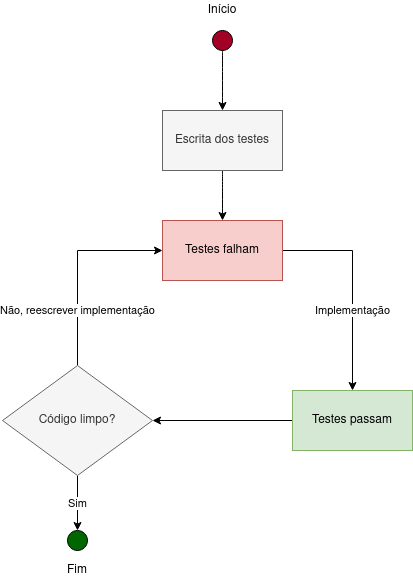
\includegraphics[scale=0.5]{img/tdd.png}
    \caption{Ciclo de desenvolvimento utilizando TDD.}
    \label{fig:tdd-cicle}
\end{figure}

\section{Teste de mutação}

Embora os testes de unidades aplicados no TDD garantam boa cobertura na base de código no sentido de satisfazer especificações de negócio, não há a garantia de que os testes estão garantindo o correto funcionamento do \textit{software}, que é o propósito principal da aplicação de testes. Ou seja, uma boa cobertura de casos de testes não garante que o \textit{software} está sendo testado adequadamente.

O Teste de Mutação de \textit{software} \cite{ieee:mutation-testing-survey} tem como objetivo proporcionar uma melhor avaliação sobre a suíte de casos de teste com base em uma pontuação de adequação. É uma técnica baseada em falhas \cite{ieee:fault-based-testing}, cuja ideia base é gerar alterações no código original, chamados de mutantes, e observar o comportamento dos testes. Por meio da técnica, o código recebe pontuação positiva se o mutante gerado faz com que algum dos testes falhem, no caso da mutação forte, ou com que as saídas sejam alteradas, no caso da mutação fraca. O objetivo principal do teste de mutação é distinguir um programa $P$, o programa correto, de um programa $P'$, o programa incorreto, utilizando-se da hipótese CPH \cite{ieee:hints-on-test-data}, que consiste na premissa de que programadores são competentes e tendem a desenvolver programas próximos do que é correto e as falhas são devidas a pequenas mudanças sintáticas no programa. As mudanças comumente utilizadas no teste de mutação podem ser listadas da forma com que se segue:

\begin{itemize}
    \item Troca de operadores lógicos, como o operador "ou", "e", "not" e "xor"
    \item Troca de operadores comparativos, como igual, diferente, maior, maior ou igual, menor e menor ou igual;
    \item Troca de operadores matemáticos, como mais, menos, produto e divisão; e
    \item Omissão ou troca de chamada de funções ou métodos.
\end{itemize}

\section{Pontos negativos do Teste de Mutação}

O uso do teste de mutação exige que para cada mutação realizada no código fonte original a suíte de casos de testes seja reexecutada novamente, fazendo com que esta técnica seja computacionalmente intensa para grandes bases de código, esse é um dos grandes pontos negativos da técnica de Teste de Mutação. Com isso, a sua aplicação no fluxo do cotidiano do desenvolvedor de \textit{software} fique inviabilizada, fazendo com que ela seja aplicada apenas em projetos cujo custo sobre falhas seja alto o suficiente.


\section{Sistemas de controle de versão de software}

Atualmente o uso de um sistema VCS se tornou algo indispensável para todo desenvolvedor de software \cite{git:review}, são ferramentas auxiliam o desenvolvedor a gerenciar o histórico de mudanças da base de código, juntar trabalhos de vários desenvolvedores, e compartilhar código fonte de forma eficiente. Um desses sistemas mais utilizados na atualidade é o Git \cite{git:website}, que possui também a característica de ser descentralizado, permitindo que o trabalho do desenvolvedor seja feita a qualquer momento, sem a necessidade de conexão com a internet para realizar mudanças na \textit{branch} local.

O fato que torna o uso desses sistemas útil para técnicas de teste de software é o de que se tem o controle de todas partes da base de código estão sendo introduzidas alterações de forma precisa, possibilitando que os testes sejam aplicados aplicados apenas nessas regiões do código fonte original.


